
\section{Specification \& Design}\label{process}

\subsection{Methodology}
In order to decide what software development framework to use when developing this app, two common Agile frameworks were considered: Scrum and Kanban. When comparing Scrum to Kanban methods, Kanban is found to often be better in terms of managing project schedules\cite{Lei2017}. It also has the following benefits: increased visibility, improved workflow, and faster time to market\cite{Ahmad2018}. Kanban boards and cards are easier to manage for a solo project compared to organising sprints, backlogs, and checkpoints for a Scrum system. Scrum also works better in teams of 3-9, not solo projects\cite{Mundra2013Practical}. Kanban has even been shown to help student manage their workload and get assignments in on time\cite{Sheng2021Kanban}. Ultimately, Kanban was chosen as the best software development framework for this project for keeping the project on schedule, workload, increasing organisation, workflow, are easy to maintain for one person, and have been proven to work in a student setting.

GitLab Issue boards were selected as the platform to host the Kanban as each issue card can be linked to branches within repositories to keep track of which tasks and changes are for which branches to improve organisation. Three labels: Code, Writing and research, and Critical, were also added to signify the type of task for each issue card. The Kanban board included four sections, one for each label and one for closed tasks. Gitlab would automatically sort each task into the relevent section based on its labels. The board was updated regularly to reflect the current status of each task, and tasks were moved from one section to another as they were completed. This resulted in tasks that were easy to prioritise, order, track, and complete on time. See Figure \ref{figure:kanban-board} for the Kanban board.

\begin{figure}[h!!]
  \begin{center}
    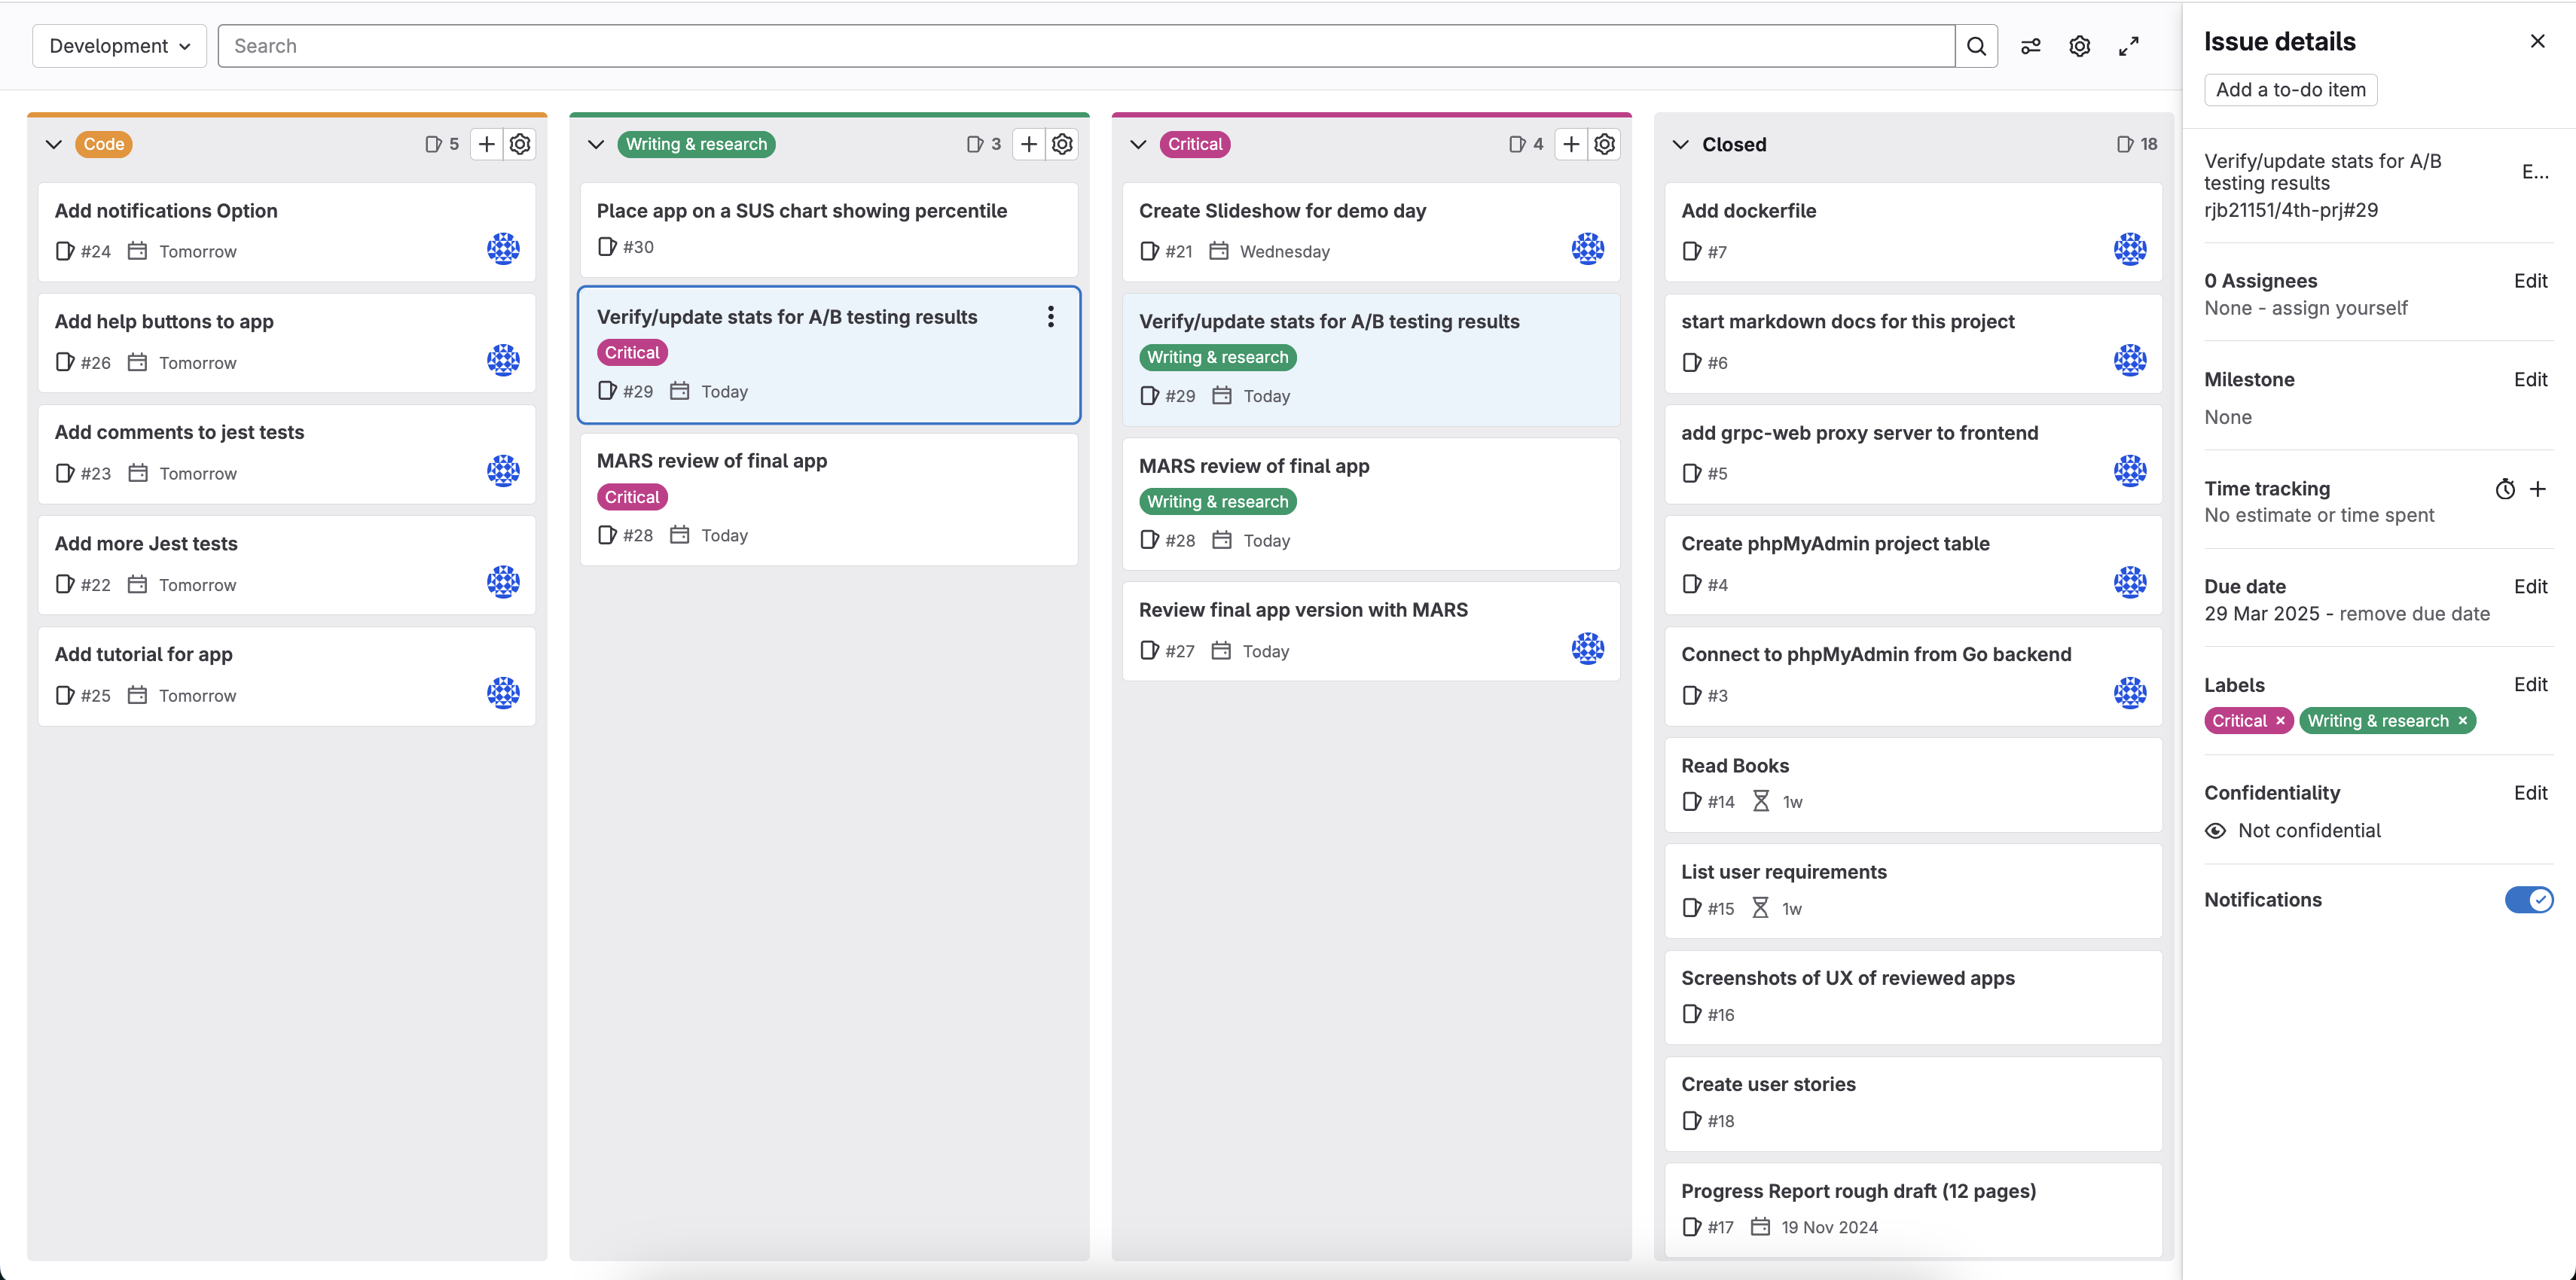
\includegraphics[scale=0.15]{Kanban.png}
    \caption{Kanban board on GitLab.}
    \label{figure:kanban-board}
  \end{center}
\end{figure}


\subsection{Mid Project Organisation}

After around a month of progress, a network diagram was made to find the critical path in order to correctly prioritise work. Once a list of the main activities was made, the dependencies of each activity were identified and the time it would take to complete each activity was estimated. The critical path was then identified by finding the path through the network diagram with a float or leeway of zero. The critical path is the sequence of activities that must be completed on time for the project to be completed on schedule. The critical path is important because it helps to identify which activities are most important for the success of the project and which activities can be delayed without affecting the overall project timeline. See Figure \ref{figure:network-diagram} for the network diagram. The critical path activities are highlighted in red. From the network diagram, it was concluded that writing the report and obtaining feedback was the most important aspect of this project and should be prioritised over other tasks. The network diagram also helped to identify potential bottlenecks in the project timeline and allowed for better planning and scheduling of tasks.

\begin{figure}[h!!]
  \begin{center}
    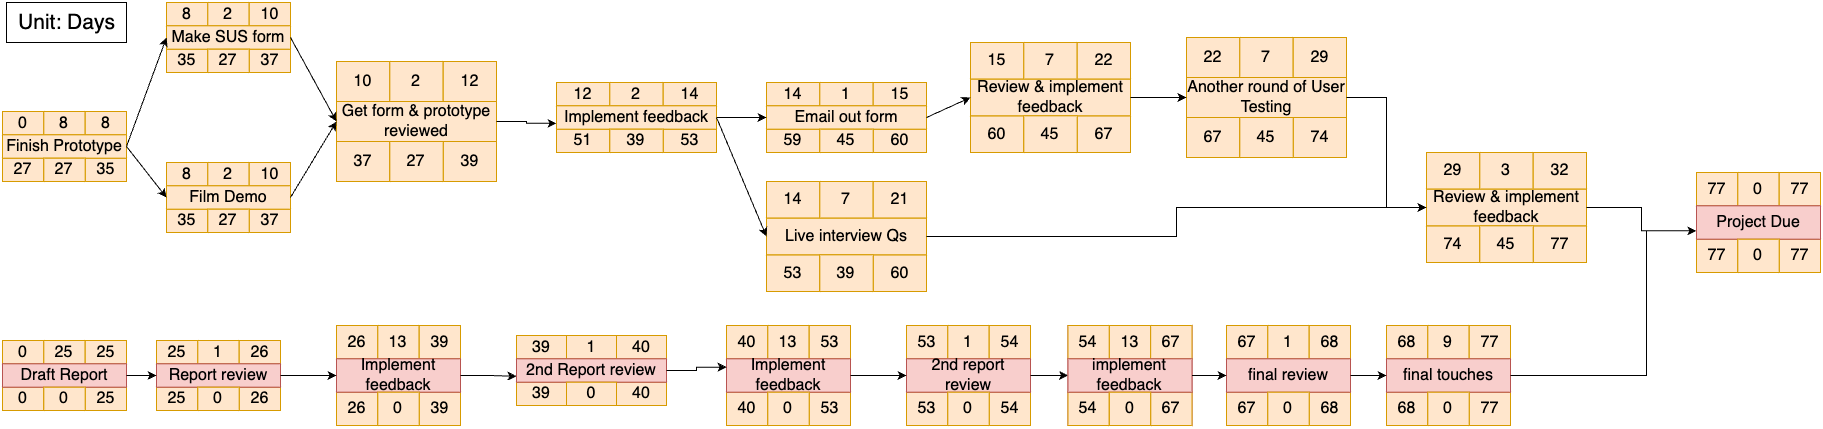
\includegraphics[scale=0.2]{NetworkDiagram.drawio.png}
    \caption{Network Diagram showing critical path.}
    \label{figure:network-diagram}
  \end{center}
\end{figure}

\subsection{Survey Specification and Design}

\subsubsection{Ethics Form}
Before beginning the process of gathering user requirements, an ethics form was drafted and completed to ensure that the research follows ethical guidelines. This Ethics form included a summary of all progress to date, included how participants were recruited, what information participants received about the study and what they were expected to do, and how user data was stored and processed. 

\subsubsection{Recruitment}
To recruit participants for the study, personal contacts in this demographic (women between the ages of 30 and 60) were invited and the supervisor for this project utilised professional and colleague email contacts and distribution lists to identify and invite women to participate. 

\subsubsection{Survey Design}
In preparation for building the product, the design and app testing stages were designed. Each testing stage involved participants completing a questionnaire via Microsoft Forms for User Requirements and app testing. 

In preparation, research was conducted through books on women’s experiences during perimenopause, including works by Kat Muir\cite{Muir2022} and Davina McCall\cite{McCall2022}, as well as reviewing research papers on health-tracking applications and a review of existing apps on the market to assess current solutions. Privacy emerged as a significant concern, with many apps engaging in surveillance capitalism and selling user data, often without informing the user or by misleading the user\cite{Gilman2021}\cite{FTC2021}. Hackers are lured to health data such as that stored by symptom tracking apps because on the black market, a person's medical data sells for 50 times what credit card information sells for\cite{Rosato2020}. This meant that the surveys must include opportunities for the users to give their opinions on privacy and their priorities in a tracking app. The first page of all online surveys conducted during the study contained the consent form with text that stated that by completing the survey, they were implying consent to take part in that phase. 

\subsubsection{User Requirements Survey Design} 
The User Requirements questionnaire contained questions regarding the users age, menopause stage, symptoms they experience, if they track their symptoms/periods, how, and the frequency of tracking. It also included questions to see if they share tracking data with their healthcare provider and if it was helpful. There were additional questions tracking challenges, triggers, menopause medication or treatment. The final questions included open ended questions about tracking frustrations, helpful aspects of tracking, challenges in understanding/identifying patterns, reminder preferences, and insights/features a user might like to see in a tracking app. 

\subsubsection{App feedback Survey Design} 

The app testing surveys were designed to gather feedback on the app's usability and user experience using a System Usability Scale (SUS) along with additional free response questions. The SUS is a widely used tool for measuring the usability of a product or system, and it consists of 10 questions that assess various aspects of the user experience\cite{Hyzy2022}. See Figure \ref{figure:sus} for the questions used in a System usability scale. The SUS scores range from 0 to 100. The score number represents the percentile the app lands in with higher scores indicating better usability. The process for calculating the SUS score involves the following steps:
\begin{enumerate}
  \item Each of the 10 questions is scored on a scale from 1 to 5, with odd-numbered questions being positively worded and even-numbered questions being negatively worded.
  \item Subtract 1 from the odd numbered questions 
  \item Subtract the users response to the even numbered questions from 5.
  \item Add the scores together and multiply by 2.5 to get the final score.
\end{enumerate}

\begin{figure}[h!!]
  \begin{center}
    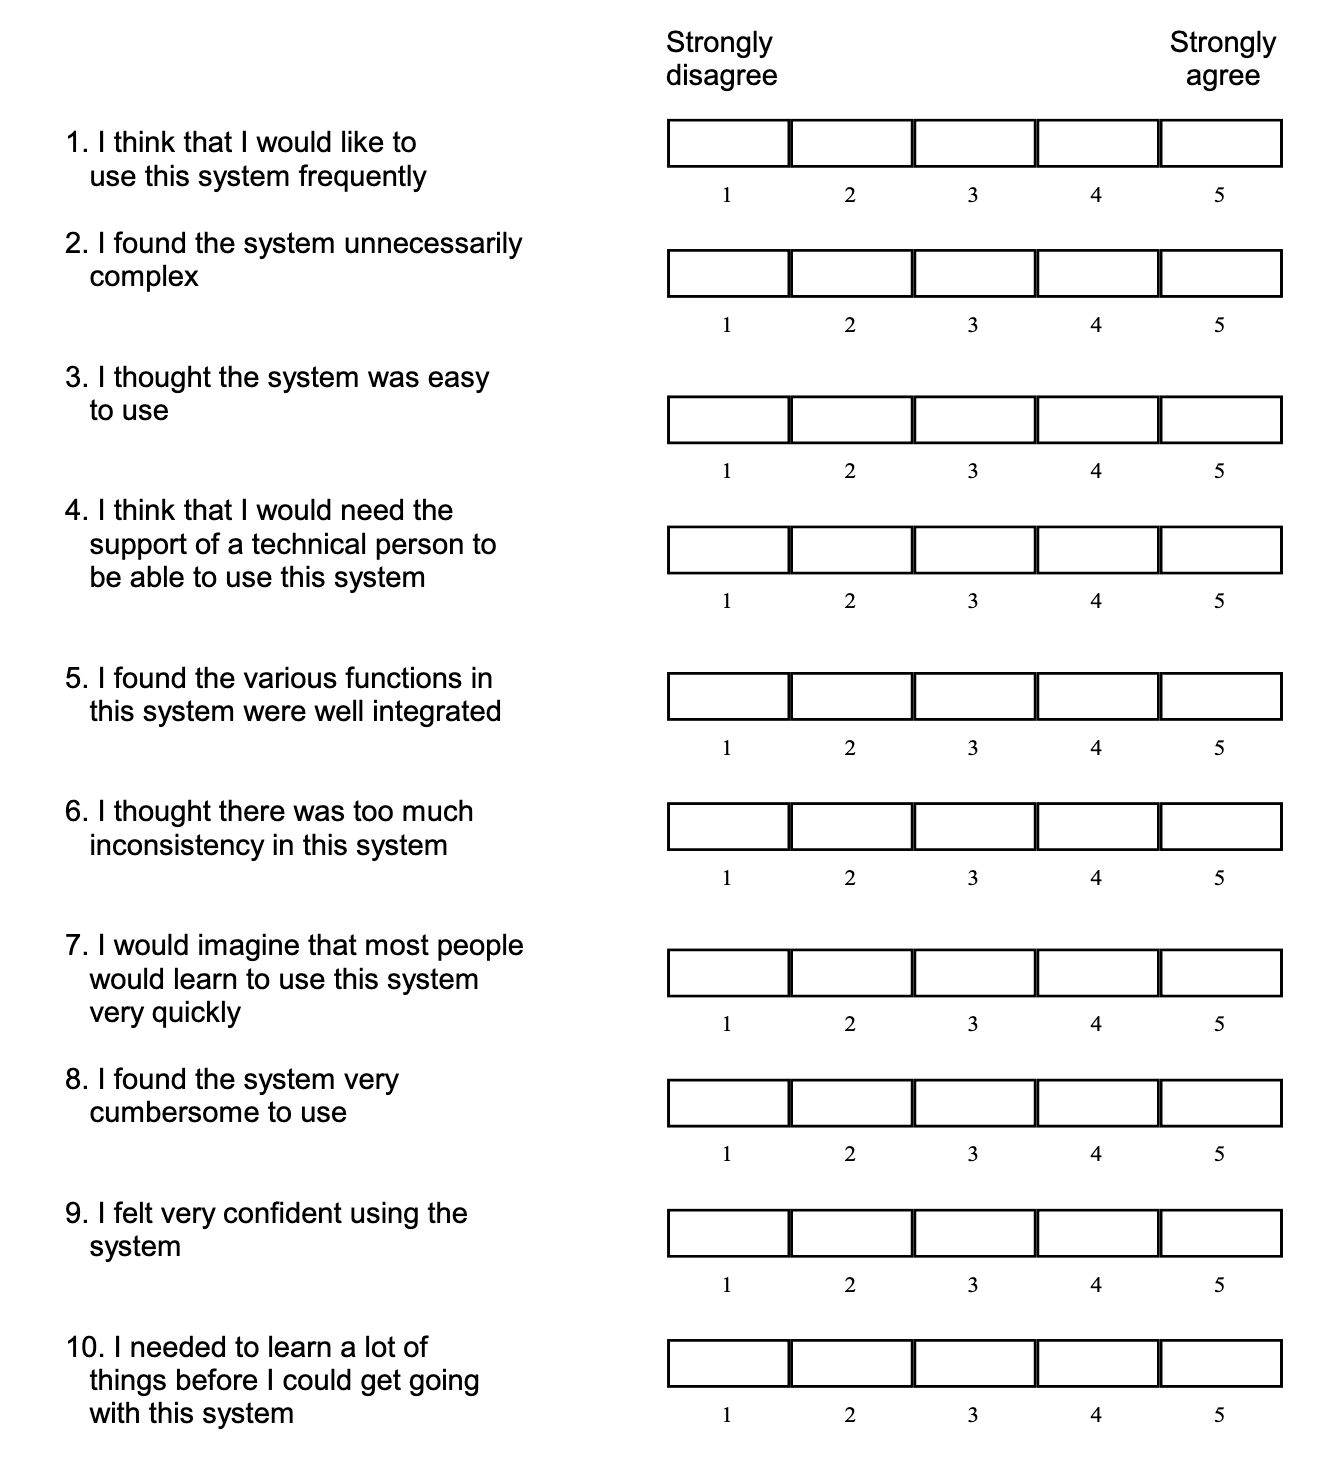
\includegraphics[scale=0.3]{SUS.png}
    \caption{System Usability Scale Questions.}
    \label{figure:sus}
  \end{center}
\end{figure}

Alternative to SUS include the User Experience Questionnaire (UEQ), the Net Promoter Score (NPS), and the System Usability Metric (SUM). The UEQ is a more comprehensive tool that assesses various aspects of user experience, including attractiveness, perspicuity, efficiency, dependability, stimulation, and novelty. The NPS measures customer loyalty and satisfaction by asking users how likely they are to recommend the product to others. The SUM is a metric that combines various usability metrics into a single score. These tools were considered for this study however these were not chosen beacuse they are not as widely used and accepted as the SUS. The SUS is a well-established and validated tool that has been used in numerous studies to assess the usability of various products and systems. It is also easy to administer and interpret, making it a practical choice for this study. The SUS is also widely recognized and accepted in the field of usability testing, which adds credibility to the findings.

The survey also included questions about the app's design, ease of use, and overall satisfaction. Participants were asked to provide open-ended feedback on what they liked and disliked about the app. The survey also included questions about the participants' demographics, such as age and experience with perimenopause, to better understand the target audience.

The app testing process was divided into 3 stages: prototype evaluation, and final app evaluation with Group A, and final app evaluation with Group B. 

The prototype evaluation was conducted using the initial React web app prototype. Since the web app was being tested locally and participants may struggle to download and let it up on their local devices, a demo video was made for users to watch. The first demo video was a screen recording of the website being used. After feedback from the project supervisor, a voiceover was added, text and zoomed in images were added, and the video was shortened to 40 seconds and edited to be more engaging. Since the video was now short and fast, the Microsoft Forms survey was edited to allow the user to rewatch the demo video as many times as they pleased. The video was then uploaded to YouTube and a link was sent to participants along with the survey. 

The second stage of evaluation for the final React Native app was conducted in an A/B testing format. Participants were divided into two equal sized groups, Group A and Group B. 
Both groups used the app for 2-5 minutes either by downloading and starting the app from a github repository or by using their iphone to scan a QR code that was linked to the app. The QR code was generated by Expo when starting the app. This allowed participants to easily access the app without having to download it from the App Store or Google Play. 

Group A got to trial the app with the initial design and features. They were asked to provide feedback on the app's usability and user experience using the SUS survey. The feedback from Group A was used to make improvements to the app before it was released to Group B. Group B then tried the app with the new design and features. They were also asked to provide feedback on the app's usability and user experience using the SUS survey. The feedback from Group B was used to make final improvements. The goal of this evaluation was to see if the changes made had a positive impact on the usability of the app. Both group A and B provided valuable feedback on the app's usability and user experience, as well as to identified areas for improvement. The Microsoft Form used for evaluation was the same for both the web and Native app for Group A and Group B. 

\subsection{Requirements}

\subsubsection{Functional Requirements}
The goal of this project is to create a user-friendly, educational, and privacy-focused perimenopausal symptom tracking app. This App's functional requirements were prioritized based on user needs and the project goal. Essential functional requirements impacting usability such as being able to navigate to a screen were prioritised over design and content details. The following functional requirements were identified from the evaluation of existing apps and from the results of the User Requirements Survey in \ref{sec:userReqResults}:

\begin{itemize}
      \item Users must be able to log the dates of their periods.
        \begin{itemize}
          \item Allowing users to track their period dates means as they enter perimenopause, they can see signs of their cycle changing and how it is changing since perimenopause is defined as a shift in mentruation patterns\cite{Brambilla1994}. 
        \end{itemize}
      \item Users must be able to log their perimenopausal symptoms and their severity daily to track changes over time.
        \begin{itemize}
          \item Perimenopause symptoms change over time and an increase in certain symptoms can signify that a women in entering or leaving the perimenopause stage\cite{Brambilla1994}.
        \end{itemize}
      \item Users must be able to edit or delete logged symptoms and period data at any time.
        \begin{itemize}
          \item 60\% of women have memory issues during perimenopause so it is cruicial that they can edit and delete symptoms and period data\cite{Gilman2021}.
        \end{itemize} 
      \item The app must store all user data locally using AsyncStorage on the users device, ensuring no data is stored on external servers.
        \begin{itemize}
          \item Since medical data is extremely valuable and often sold or stolen, privacy is an extremly important aspect of this app\cite{Gilman2021}\cite{Rosato2020}.
        \end{itemize}
      \item The app must include a calendar view where users can see logged symptoms and period data over time. The app must provide graph-based visualizations showing symptom frequency and period heaviness trends over time.
        \begin{itemize}
          \item Calendars allows users to see patterns in their symptoms and period data over time, which can help them identify triggers and patterns\cite{Brambilla1994}.
        \end{itemize}
      \item The app must provide an option to reset user data to align with privacy-focused design principles
        \begin{itemize}
          \item Users should be able to delete their data if they no longer want to use the app or if they are concerned about privacy since one of the goals of this project is to be privacy focused.
        \end{itemize}
      \item The app must calculate and display the most common symptom based on user entries.
        \begin{itemize}
          \item This allows users to see which symptoms are most common for them and can help them identify treatment when talking to their doctor\cite{Brambilla1994}.
        \end{itemize}
      \item The app must provide cycle length insights based on logged period data.
        \begin{itemize}
          \item This allows users to compare their cycle length to the average premenopausal cycle to help them classify what stage of menopause they may be in or show their doctors\cite{Brambilla1994}.
        \end{itemize}
      \item The app must calculate average period length based on tracked cycles.
        \begin{itemize}
          \item This allows users to compare their period duration to the average period duration to help inform them what stage of menopause they may be in or show their doctors\cite{Brambilla1994}.
        \end{itemize}
      \item Users must be able to access an Analysis Tab summarizing trends.
        \begin{itemize}
          \item This allows users to see patterns in their symptoms and period data over time, which can help identify irregularities\cite{Brambilla1994}.
        \end{itemize}
      \item The app must feature a Learn Page with information on perimenopause and related topics. Users must be able to access external links to trusted resources for more detailed information.
        \begin{itemize}
          \item Since menopause is rarely talked about in media, is a taboo topic, and most women and many doctors are never educated on it, providing a source of reliable information about menopause is crucial to help women understand their symptoms and how to manage them\cite{Aljumah2023}\cite{MenopauseSupport2021}\cite{Muir2022}.
        \end{itemize}
      \item The app must follow EU accessibility standards, including text scaling, color contrast, and screen reader compatibility.
        \begin{itemize}
          \item  Many women experience blurred vision during perimenopause and menopause since as estrogen levels fall, the cornea things and becomes less elastic which impacts the ability to focus light and causes blurred vision. Because of this, it is extremely important that the app accomodates those with impaired vision by having large text mode and high contrast modes\cite{KellyDonel2023}.
        \end{itemize}      
\end{itemize}

\subsubsection{Non-Functional Requirements}
There are well-established industry standards for the non-functional requirements of Apps\cite{Apple2025}\cite{Tundwal2025}. The key topics for non functional requirements touch on performance, security, usability, comptaibility, reliability, and maintainability. The most relevant ones for this project are:

\begin{itemize}
  \item The time taken by the app to respond to user input should be minimal
  to ensure a smooth user experience\cite{Tundwal2025}.
  \item The time taken for the app to start up should be optimized to prevent
  user drop-off\cite{Tundwal2025}.
  \item The app should handle increases in load without a
  significant drop in performance\cite{Tundwal2025}.
  \item The app must run on the currently shipping OS\cite{Apple2025}.
  \item Apps must request explicit user consent and provide a clear visual
  and/or audible indication when recording, logging, or otherwise making a
  record of user activity\cite{Apple2025}.
  \item Widgets, extensions, and notifications should be related to the
  content and functionality of your app\cite{Apple2025}.
  \item Apply code hardening techniques and obfuscate the code to make it
  harder for attackers to analyze and exploit the app.\cite{Tundwal2025}.
  \item Create an intuitive user interface that allows users to navigate easily and accomplish tasks without confusion\cite{Tundwal2025}.
  \item Use high contrast colors and allow font size adjustments to improve readability for users with visual impairments\cite{Tundwal2025}.
  \item The app should comply with WCAG 2.2 level AA guidelines and standards to maintain acessibility\cite{GovUK_WCAG}.
\end{itemize}

As the project developed, user requirements were designed to be continually adjusted to best reflect the goal of this project.


\subsection{Design}
To meet the user-friendly goal, the design of the App's user interface went through multiple iterations, informed by user feedback.

\subsubsection{Interface Design}
At the beginning of the design process, low fidelity wireframes were created using Figma (See Figure \ref{figure:figma-1}).
\begin{figure}[h!!]
  \begin{subfigure}{.5\textwidth}
    \begin{center}
      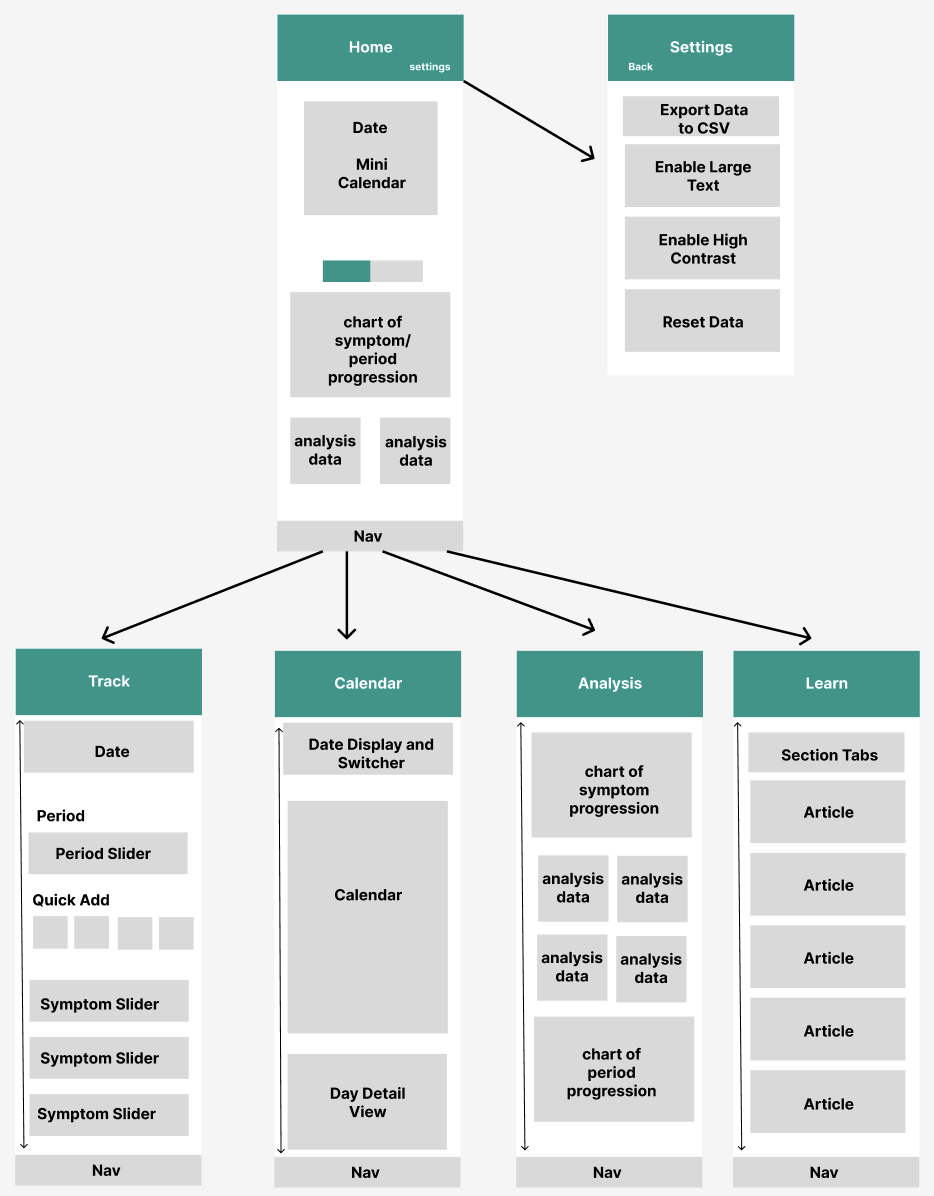
\includegraphics[scale=0.3]{Figma-1.png}
      \caption{Wireframe of App on Figma.}
      \label{figure:figma-1}
    \end{center}
  \end{subfigure}
  \begin{subfigure}{.5\textwidth}
    \begin{center}
      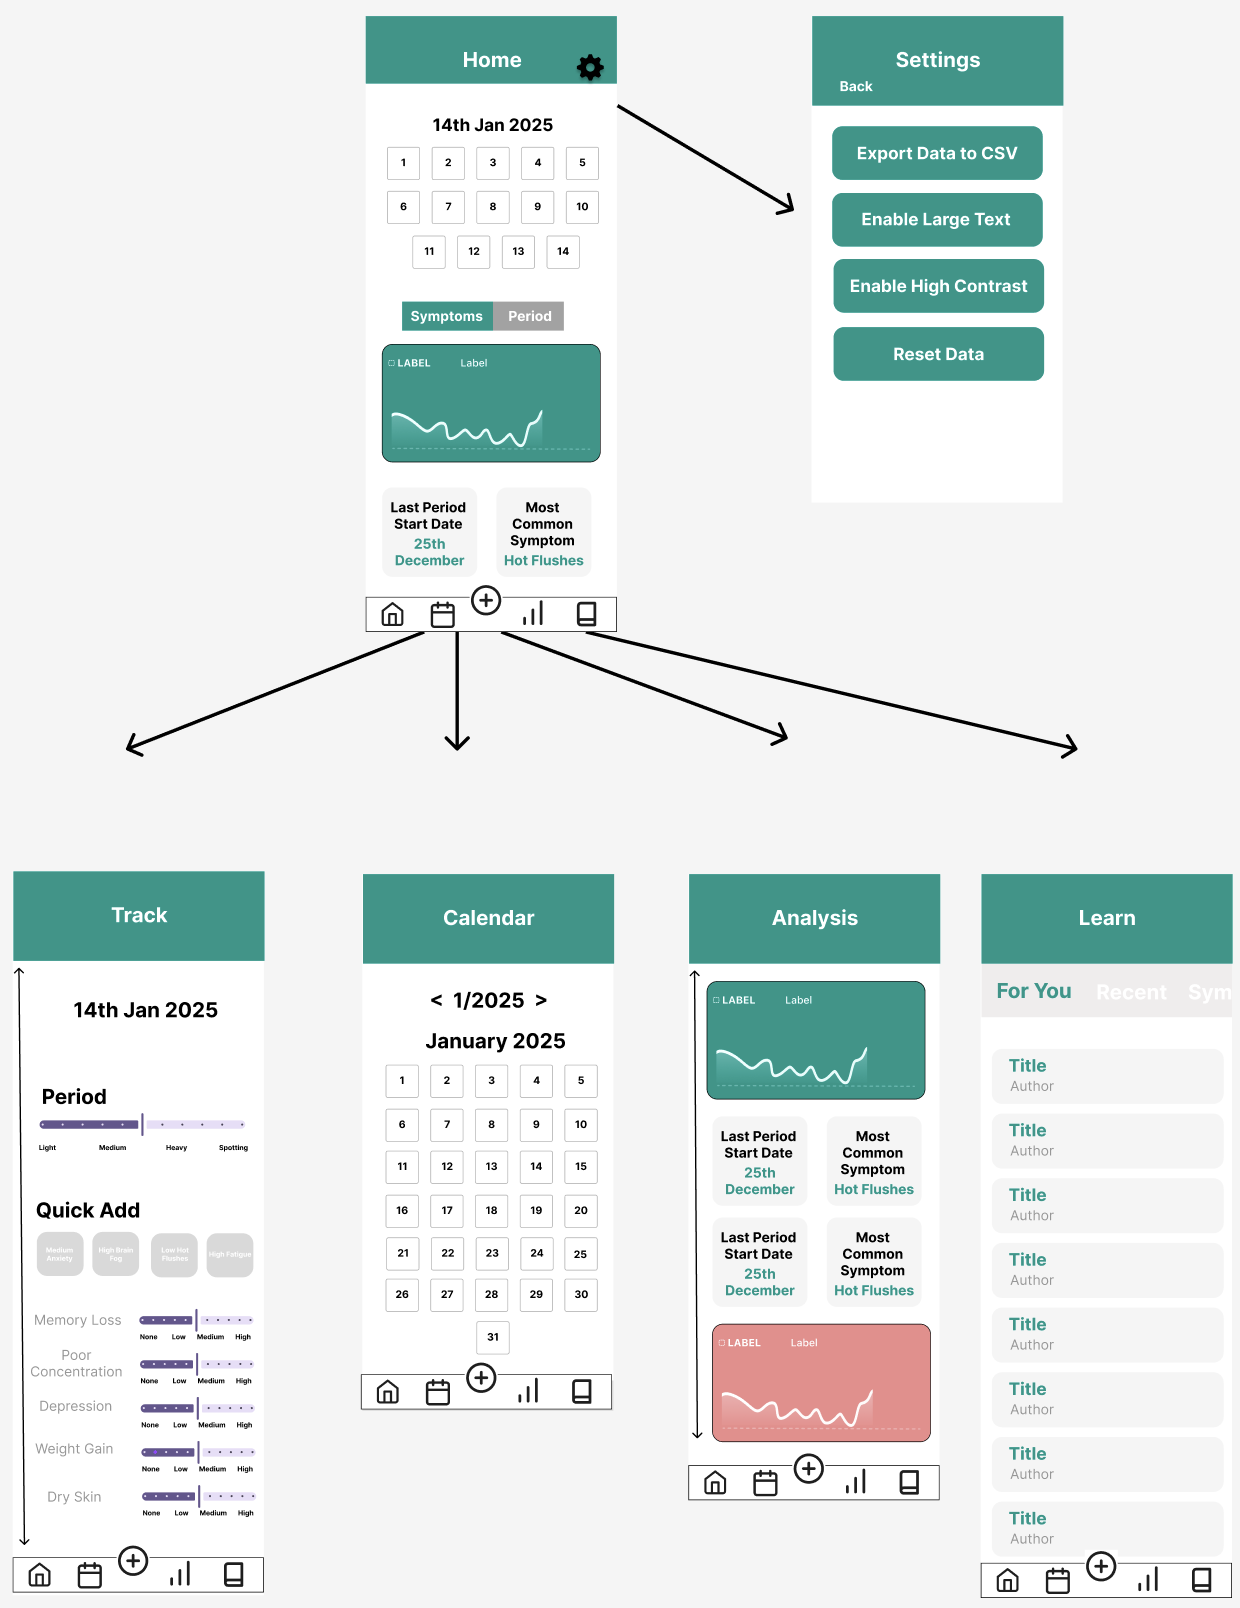
\includegraphics[scale=0.25]{Figma-2.png}
      \caption{Detailed Draft of App on Figma.}
      \label{figure:figma-2}
    \end{center}
  \end{subfigure}
\end{figure}

The colour scheme was chosen to be relaxing and calming  through the use of blue and green tones. The app was designed to be user-friendly and intuitive, with a focus on simplicity and ease of use. The design was also created with the goal of making it easy for users to navigate the app and find the information they need, as well as be responsive and work well on different screen sizes, including tablets and smaller phones. The design was then fleshed out into a more detailed figma design. See Figure \ref{figure:figma-2}.

The final design as seen in figure\ref{figure:app} was created with a focus on simplicity and ease of use. The app was designed to be user-friendly and intuitive, with a clean and simple design. The final color scheme was chosen to be calming and easy on the eyes, with a focus on blues and greens. Feedback from user evaluations was incorporated into the design to ensure that it met the needs of the target audience. Some user feedback that was implemented includes adding days of the week to the mini calendar in the home page, making the track button in the nav bar larger and a different color to make it more visible, ability to refresh the home page, and ability to track by clicking a day in the calendar. 
\begin{figure}[h!!]
  \begin{center}
    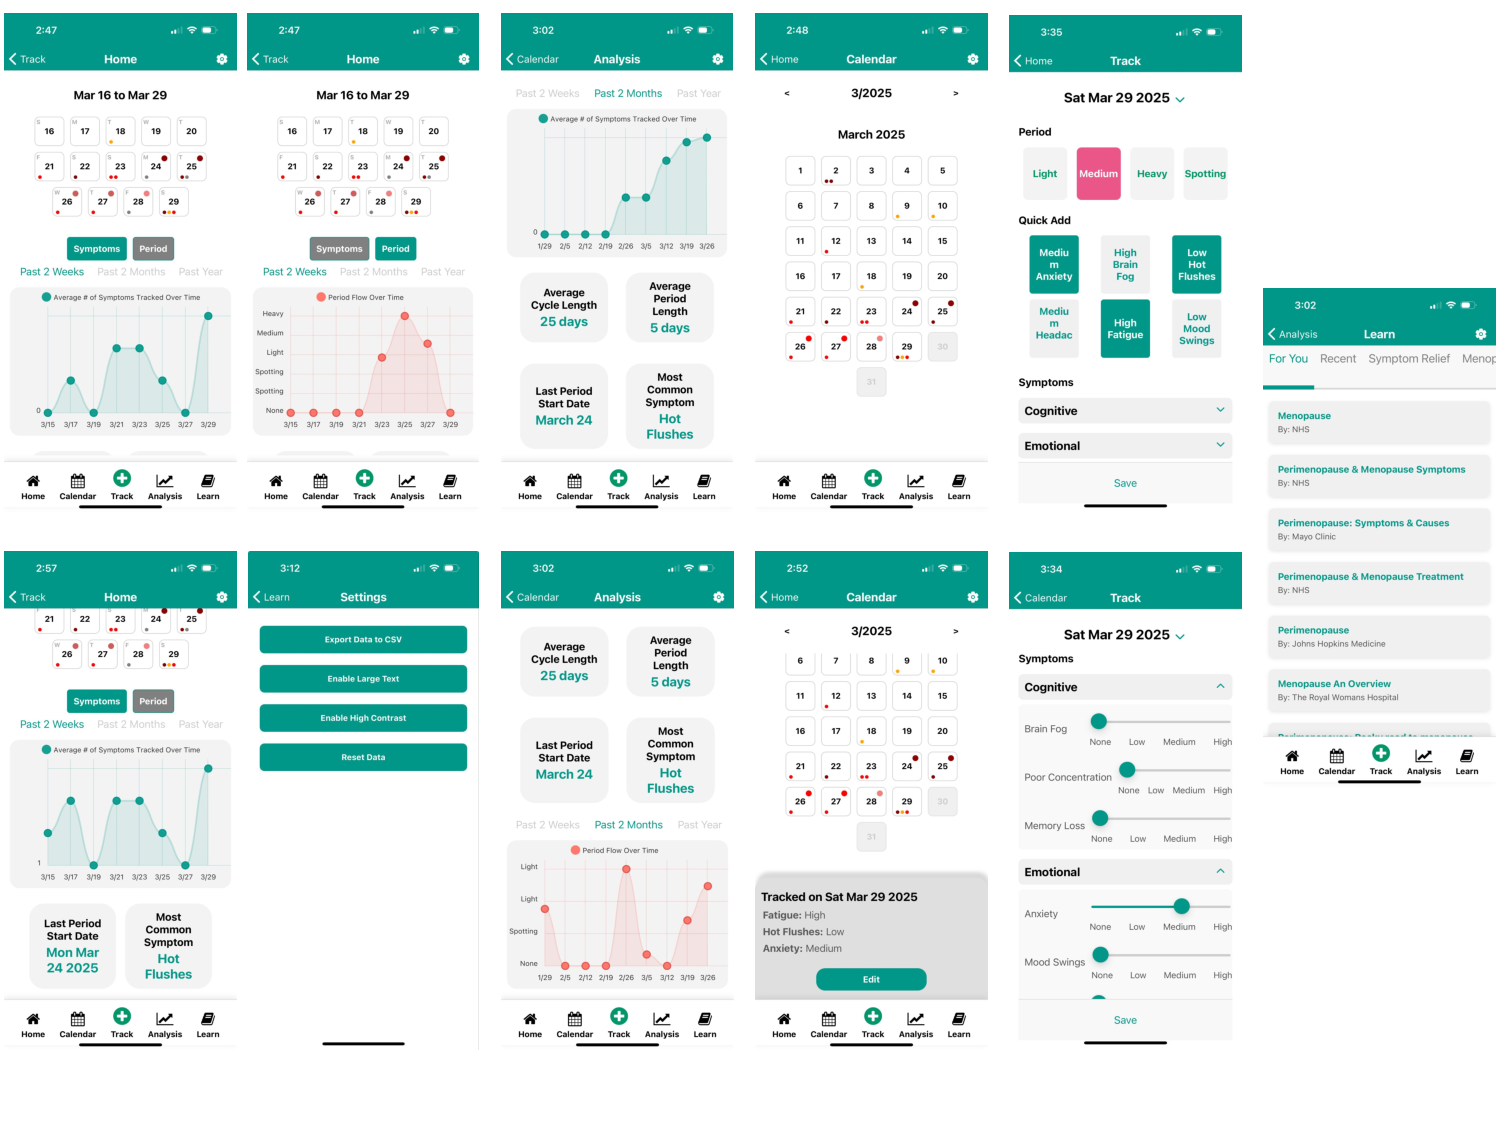
\includegraphics[scale=0.4]{app.pdf}
    \caption{Final React Native App Design.}
    \label{figure:app}
  \end{center}
\end{figure}

The app was then compared to the EU WAG 2.1 accessibility standards and adjusted to be accessible to all users, with large text and color contrast options in the settings. Figure \ref{figure:app-Accessible} shows the app in dark mode with high contrast and large text mode enabled.
\begin{figure}[h!!]
  \begin{center}
    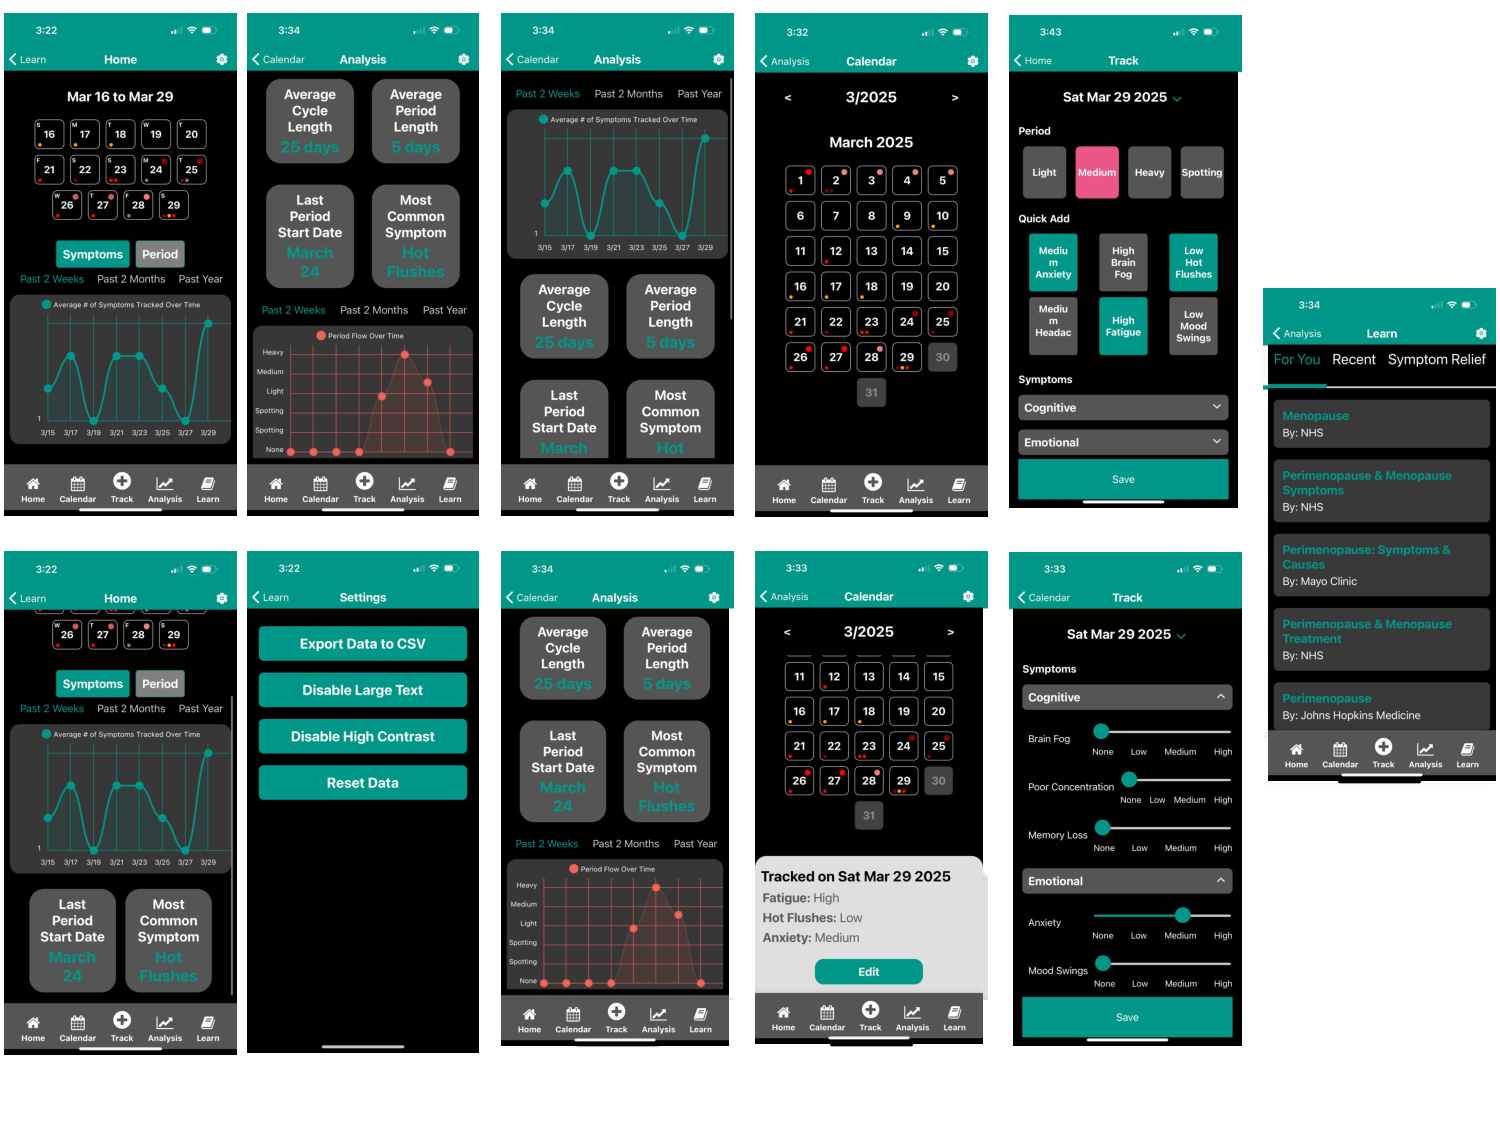
\includegraphics[scale=0.4]{app-Accessible.pdf}
    \caption{Final React Native App Design with high contrast and large text on.}
    \label{figure:app-Accessible}
  \end{center}
\end{figure}

\subsubsection{System Design}
In the interest of protecting user privacy, there is no database and all data is stored on the user's local device. The data that is saved in AsyncStorage on their device is formatted as featured in table\ref{table:user-data}. 
\begin{table}[h!!]
    \caption{Structure of User Data Stored in AsyncStorage}
    \label{table:user-data}
    \begin{tabular}{llll}
    \hline
    Anonymous User &        &          &          \\ \hline
                  & Date1  &          &          \\
                  &        & Symptom1 & Severity \\
                  &        & Symptom2 & Severity \\
                  & Date2  &          &          \\
                  &        & Symptom1 & Severity \\
                  &        & Symptom2 & Severity \\
                  & Date n &          &          \\
                  &        & Symptom1 & Severity \\
                  &        & Symptom2 & Severity \\ \hline
  \end{tabular}
\end{table}

The data is stored using JSON as that is the required format specified by Async Storage. JSON (JavaScript Object Notation) is a lightweight data interchange format that is easy for humans to read and write, and easy for machines to parse and generate\cite{JSON2025}. The data is stored in a dictionary format with the date as the key and the symptoms and their severity as the values. The severity is stored as a number from 1-5, with 1 being not severe and 5 being extremely severe. This allows for easy access to the data and makes it easy to display in graphs and charts. The data is also stored in a way that is easy to update and delete.

The list of perimenopause symptoms is also structured in the same way as user data. There is a JSON file with ``symptoms'' as the top level object. Each symptom is then stored with the display name as the value and a version of the symptom with no spaces or capitals is used as the key. This allows for easy access to the symptoms and makes it easy to display in the app. The symptoms are also stored in a way that allows for easy editing and deletion of symptoms. This file is small and acessed frequently so it is stored in the app bundle and not Async Storage.

For each json structure (articles, symptoms, and userData), there is a relevant JSON Schema to validate the objects. A JSON schema is used to validate JSON data to ensure validity, consistency, correct structure, and valid data types\cite{JsonSchema2025}\cite{JsonSchemaOrg2025}. Each schema is in the root directory of the project and ends in ''.schema.json''. The JSON Schema Validator is used to show validation issues in the problems tab of VS code during development to highlight any issues with the JSON structure and make it easier to debug.